%%%%%%%%%%%%%%%%%%%%%%%%%%%%%%%%%%%%%%%%%%%%%%%%%%
% Adam Newton Wright
% Senior Thesis Presentation Fall 2017
% 11.24.2017
% senior_presentation_fall.tex
%%%%%%%%%%%%%%%%%%%%%%%%%%%%%%%%%%%%%%%%%%%%%%%%%%



\documentclass{beamer}
\beamertemplatenavigationsymbolsempty
\usepackage{graphicx} 
\usepackage{animate}
\usepackage{siunitx}
\usepackage{tikz}
%\usepackage{standalone}
\usepackage{color}
\newcommand{\btVFill}{\vskip0pt plus 1filll}
\usepackage[export]{adjustbox} 
\usetheme{Szeged}
\usecolortheme{wolverine}
\usepackage{wrapfig}
%Information to be included in the title page:
\title{Improving Laser Guide Stars through \\Magnetic Resonant Pulsing}
\author{Adam Newton Wright}
\institute{Willamette University}
 
\begin{document}




%%%%%%%%%%%%%%%%%%%%%%%%%%%%%%%%%%%%%%%%%%%%%%%%%%
% Title Slide
%%%%%%%%%%%%%%%%%%%%%%%%%%%%%%%%%%%%%%%%%%%%%%%%%%
{
	\usebackgroundtemplate{\includegraphics[width=\paperwidth,height=\paperheight]{Images/lgs_livermore.jpg}}
	\begin{frame}
	  \color{white}
	  \titlepage
	  \bigskip
	  \btVFill
	  {\tiny{Bishop, Brianna, ``Bringing New Life to Laser Guide Star,''Lawrence Livermore National Laboratory, June 2014}}

	\end{frame}
 } 




%%%%%%%%%%%%%%%%%%%%%%%%%%%%%%%%%%%%%%%%%%%%%%%%%%
% Overview
%%%%%%%%%%%%%%%%%%%%%%%%%%%%%%%%%%%%%%%%%%%%%%%%%%
  
\tikzstyle{decision} = [diamond, draw, fill=blue!20, 
    text width=4.5em, text badly centered, node distance=3cm, inner sep=0pt]
\tikzstyle{block} = [rectangle, draw, fill=blue!20, 
    text width=20em, text centered, rounded corners, minimum height=3em]
\tikzstyle{line} = [draw, -latex']
\tikzstyle{cloud} = [draw, ellipse,fill=red!20, node distance=3cm,
    minimum height=2em]


\begin{frame}{Overview}
\center
\vspace{-.5cm}
\begin{tikzpicture}[node distance = 2cm, auto]
    % Place nodes
    \node [block] (lgs) {Laser Guide Stars};
    \node [block, below of=lgs] (mrp) {Improving Laser Guide Stars};
    \node [block, below of=mrp] (exp) {Our Experiment};
    % Draw edges
    %\path [line] (init) -- (identify);
	\draw[->, line width = 3pt] (lgs) -- (mrp);
	\draw[->, line width = 3pt] (mrp) -- (exp);
\end{tikzpicture}
\end{frame}

{
	\usebackgroundtemplate{\includegraphics[width=\paperwidth,height=\paperheight]{Images/lgs_livermore.jpg}}
	\begin{frame}
	  \color{white}
	  \bigskip
	  \btVFill
	  {\tiny{Bishop, Brianna, ``Bringing New Life to Laser Guide Star,''Lawrence Livermore National Laboratory, June 2014}}

	\end{frame}
 } 

%%%%%%%%%%%%%%%%%%%%%%%%%%%%%%%%%%%%%%%%%%%%%%%%%%
% Atmospheric Distortion Example
%%%%%%%%%%%%%%%%%%%%%%%%%%%%%%%%%%%%%%%%%%%%%%%%%%
\begin{frame}
  \frametitle{Telescopic Imaging}
  \framesubtitle{Concerned with Highest Resolution}
  \center
  \includegraphics[scale = .3]{Images/galaxywoao.png}
	  \bigskip
	  \btVFill

\end{frame}


%%%%%%%%%%%%%%%%%%%%%%%%%%%%%%%%%%%%%%%%%%%%%%%%%%
% Atmospheric Distortion
%%%%%%%%%%%%%%%%%%%%%%%%%%%%%%%%%%%%%%%%%%%%%%%%%%
\begin{frame}
  \frametitle{Atmospheric Distortion}
  \framesubtitle{Causes reduced quality in telescopic imaging}
  \center
  \includegraphics[width = .9\textwidth]{../Thesis/FullPaper/Images/tikz/atmdistortion}
  %{\tiny $^1$Wizinowich, "The WM Keck Observatory laser guide star adaptive optics system: overview." Publications of the Astronomical Society of the Pacific 118, no. 840 (2006): 297.}
\end{frame}


%%%%%%%%%%%%%%%%%%%%%%%%%%%%%%%%%%%%%%%%%%%%%%%%%%
% Laser Guide Stars: What are they
%%%%%%%%%%%%%%%%%%%%%%%%%%%%%%%%%%%%%%%%%%%%%%%%%%
\begin{frame}
  \frametitle{Laser Guide Stars}
  \framesubtitle{Aid in correcting distorted images through adaptive optics$^{2}$}
  \begin{minipage}{.45\textwidth}
		  \includegraphics[width = 4cm, height = 5.5cm]{Images/lgs_insky.jpg}
  \end{minipage}
  \begin{minipage}{.45\textwidth}
		  \center
  	\begin{tikzpicture}
		\node() at (0,4.5);
			\draw[] (0:1) arc (0:180:1) node at (0,.25) {Earth};
			\draw[] (45:2.5) arc (45:180-0:2.5) node at (0,1.75) {Troposphere};
			\draw[] (45:4) arc (45:180-0:4) node at (0,3.25) {Stratosphere};
			\draw[] (45:5.5) arc (45:180-0:5.5) node at (0,4.55) {Mesosphere};
			\draw[-stealth] (180-15:1) -- (180-15:2.5) node at (180-5:1.75) {10 km};
			\draw[-stealth] (180-30:1) -- (180-30:4) node at (180-25:3.25) {50 km};
			\draw[-stealth] (180-45:1) -- (180-45:5.5) node at (180-35:5) {80 km};
  	\end{tikzpicture}
  \end{minipage}
	  \btVFill
	  {\tiny  $^2$``Laser Guide Star,'' RP Photonics, 2016}\\
	  {\tiny ``Laser-Guide Star HD Videos and Imagesi,`` Gemini Observatory/AURA, gemini.edu, 2013 }
\end{frame}

%%%%%%%%%%%%%%%%%%%%%%%%%%%%%%%%%%%%%%%%%%%%%%%%%%
% Adaptive Optics
%%%%%%%%%%%%%%%%%%%%%%%%%%%%%%%%%%%%%%%%%%%%%%%%%%
\begin{frame}{Adaptive Optics}
  \framesubtitle{Correct distortions from atmosphere}
		\vspace{-.3cm}
		\center
		\includegraphics[width=0.8\textwidth]{Images/AOfigure.jpg}
		\btVFill
	\vspace{-.1cm}
		{\tiny C. Max, Center for Adaptive Optics, Lawrence Livermore National Laboratory and NSF Center for Adaptive Optics, 2016}
\end{frame}

%%%%%%%%%%%%%%%%%%%%%%%%%%%%%%%%%%%%%%%%%%%%%%%%%%
% Correction with AO
%%%%%%%%%%%%%%%%%%%%%%%%%%%%%%%%%%%%%%%%%%%%%%%%%%

\begin{frame}{Adaptive Optics and LGS}
  \framesubtitle{Correct distortions from atmosphere}
  \center
  \vspace{-1.6cm}
  \animategraphics[scale = .35,autoplay,loop]{7}{AOmovie/aomovie_hist}{}{}
\end{frame}



\begin{frame}{Adaptive Optics and LGS}
  \framesubtitle{Correct distortions from atmosphere}
  \center
 \begin{minipage}{0.45\textwidth}
		  \centering
			\includegraphics[width=1.0\textwidth]{Images/galaxywoao.png}
	\end{minipage}
	\begin{minipage}{0.45\textwidth}
			\centering
			\includegraphics[width=1.0\textwidth]{Images/galaxywao.png}
	\end{minipage}	
\end{frame}



%%%%%%%%%%%%%%%%%%%%%%%%%%%%%%%%%%%%%%%%%%%%%%%%%%
% Geomagnetic Field
%%%%%%%%%%%%%%%%%%%%%%%%%%%%%%%%%%%%%%%%%%%%%%%%%%
\begin{frame}
  \frametitle{Geomagnetic Field}
  \framesubtitle{Reduces the benefits of Optical Pumping$^{5}$}
  \centering
  \begin{figure}
		  \vspace{-.5cm}
	\includegraphics[scale = .5]{Images/magneticfield.jpg}
	\end{figure}
	\vspace{-1cm}
  {\tiny $^5$Rampy, Rachel, Donald Gavel, Simon M. Rochester, and Ronald Holzlöhner. "Toward optimization of pulsed sodium laser guide stars." JOSA B 32, no. 12 (2015): 2425-2434.}\\
  {\tiny TesTeach.com, Geomagnetic Field}

\end{frame}


%%%%%%%%%%%%%%%%%%%%%%%%%%%%%%%%%%%%%%%%%%%%%%%%%%
% Larmor Precession
%%%%%%%%%%%%%%%%%%%%%%%%%%%%%%%%%%%%%%%%%%%%%%%%%%
\begin{frame}
  \frametitle{Optical Pumping}
  \framesubtitle{Larmor Precession}
  %\vspace{-.4cm}
	  \begin{minipage}{0.4\textwidth}
		\vspace{-5cm}
	  \begin{center}
		 $\vec \tau = \vec \mu \times \vec B $\\
	\vspace{1cm}
	   $\omega = -\gamma B$\\
	\vspace{1cm}
	   $ \gamma = \frac{eg}{2m}$
	\end{center}
  \end{minipage}
  \hfill
  \begin{minipage}[b]{0.4\textwidth}
	  \begin{tikzpicture}
		  \node at (0,0) {\includegraphics[scale = .4]{Images/larmorprecession.png}};
		  \node at (0,3) {\Large$\vec B$};
		  \node at (1,1) {\Large$\vec \mu$};
		  \node at (1,2.3) {\Large$\omega$};
	  \end{tikzpicture}
  \end{minipage}
	%\\\scriptsize{where $\tau$ is the torque exerted, $\mu$ is the magnetic dipole moment, $B$ is the external magnetic field, $\omega$ is the angular frequency, and $\gamma$ is the gyromagnetic ratio with $e$ being the electric charge, $g$ being the \textit{g-factor}, and $m$ being the mass of the object.}
\end{frame}



%%%%%%%%%%%%%%%%%%%%%%%%%%%%%%%%%%%%%%%%%%%%%%%%%%
% Larmor Precession
%%%%%%%%%%%%%%%%%%%%%%%%%%%%%%%%%%%%%%%%%%%%%%%%%%
\begin{frame}{Larmor Precession}
\framesubtitle{}
  \animategraphics[scale = .8,autoplay,loop]{6}{MRgifd/precession}{}{}
\end{frame}



%%%%%%%%%%%%%%%%%%%%%%%%%%%%%%%%%%%%%%%%%%%%%%%%%%
% Continuous pulsing gif
%%%%%%%%%%%%%%%%%%%%%%%%%%%%%%%%%%%%%%%%%%%%%%%%%%
\begin{frame}{Continuous Wave Pumping}
  \framesubtitle{}
  \animategraphics[scale = .8,autoplay,loop]{6}{MRgifd/contpic}{}{}
\end{frame}

%%%%%%%%%%%%%%%%%%%%%%%%%%%%%%%%%%%%%%%%%%%%%%%%%%
% Magnetic Resonant Pulsing GIF
%%%%%%%%%%%%%%%%%%%%%%%%%%%%%%%%%%%%%%%%%%%%%%%%%%
\begin{frame}{Magnetic Resonant Pulsing}
  \framesubtitle{}
  \animategraphics[scale = .8,autoplay,loop]{6}{MRgifd/mrpic}{}{}
\end{frame}




%%%%%%%%%%%%%%%%%%%%%%%%%%%%%%%%%%%%%%%%%%%%%%%%%%
% Hypothesis
%%%%%%%%%%%%%%%%%%%%%%%%%%%%%%%%%%%%%%%%%%%%%%%%%%
\begin{frame}{Expected Results}
	%\frametitle{Expected Results}
  \framesubtitle{Polarization Switching}
  \centering
  \includegraphics[width=0.8\textwidth]{../Thesis/FullPaper/Images/polarizationswitch.png}
\vspace{-.3cm}
{\\\tiny Fan Improving Sodium LGS through Polarization Switching, Scientific Papers}
\end{frame}

\begin{frame}
  \frametitle{Expected Results}
  \framesubtitle{Magnetic Resonant Pulsing}
  \begin{center}
	\begin{tikzpicture}
	  \node at (0,0) {\includegraphics[width = .8\textwidth]{Images/hilmangraph1.png}};
	  \node at (-4.5,0) [rotate = 90] {Emission $Wm^{-2}$};
	  \node at (0,-3) {Angle between $\vec B$ and laser beam};
  \end{tikzpicture}
\end{center}
\vspace{-.5cm}
{\tiny Kane, "Pulsed laser architecture for enhancing backscatter from sodium." SPIE Astronomical Telescopes.}
\end{frame}



%%%%%%%%%%%%%%%%%%%%%%%%%%%%%%%%%%%%%%%%%%%%%%%%%%
% Experimental Overview
%%%%%%%%%%%%%%%%%%%%%%%%%%%%%%%%%%%%%%%%%%%%%%%%%%
\begin{frame}
  \frametitle{Our Experiment}
  \framesubtitle{Outline}
  \center
\begin{tikzpicture}[node distance = 1.75cm, auto]
    % Place nodes
    \node [block] (mrpdye) {Create Pulsed Laser};
    \node [block, below of=mrpdye] (Rb) {Magnetic Field and Rb Confinement};
    \node [block, below of=Rb] (Sp) {Fluorescence Measurements};
	\draw [->, line width = 3pt] (mrpdye) -- (Rb);
	\draw [->, line width = 3pt] (Rb) -- (Sp);
\end{tikzpicture}
\end{frame}

%%%%%%%%%%%%%%%%%%%%%%%%%%%%%%%%%%%%%%%%%%%%%%%%%%
% Laser System
%%%%%%%%%%%%%%%%%%%%%%%%%%%%%%%%%%%%%%%%%%%%%%%%%%
\begin{frame}{Laser System}
\framesubtitle{Created with diode laser and AOM}
\centering
	\includegraphics[width=0.8\textwidth]{../Thesis/FullPaper/Images/diodepulse.pdf}
\end{frame}





%%%%%%%%%%%%%%%%%%%%%%%%%%%%%%%%%%%%%%%%%%%%%%%%%%
% Magnetic Field Chamber
%%%%%%%%%%%%%%%%%%%%%%%%%%%%%%%%%%%%%%%%%%%%%%%%%%
\begin{frame}
  \frametitle{Our Experiment}
  \framesubtitle{Rubidium Housing and Magnetic Field}
  \centering
  \includegraphics[width = .9\textwidth]{../Thesis/FullPaper/Images/tikz/fluorescence}
\end{frame}


\begin{frame}
  \frametitle{Our Experiment}
  \framesubtitle{Rubidium Housing and Magnetic Field}
  \centering
  \includegraphics[width = .8\textwidth]{../Thesis/FullPaper/Images/tikz/FlvsAngle}
\end{frame}

\begin{frame}
  \frametitle{Our Experiment}
  \framesubtitle{Rubidium Housing and Magnetic Field}
  \centering
  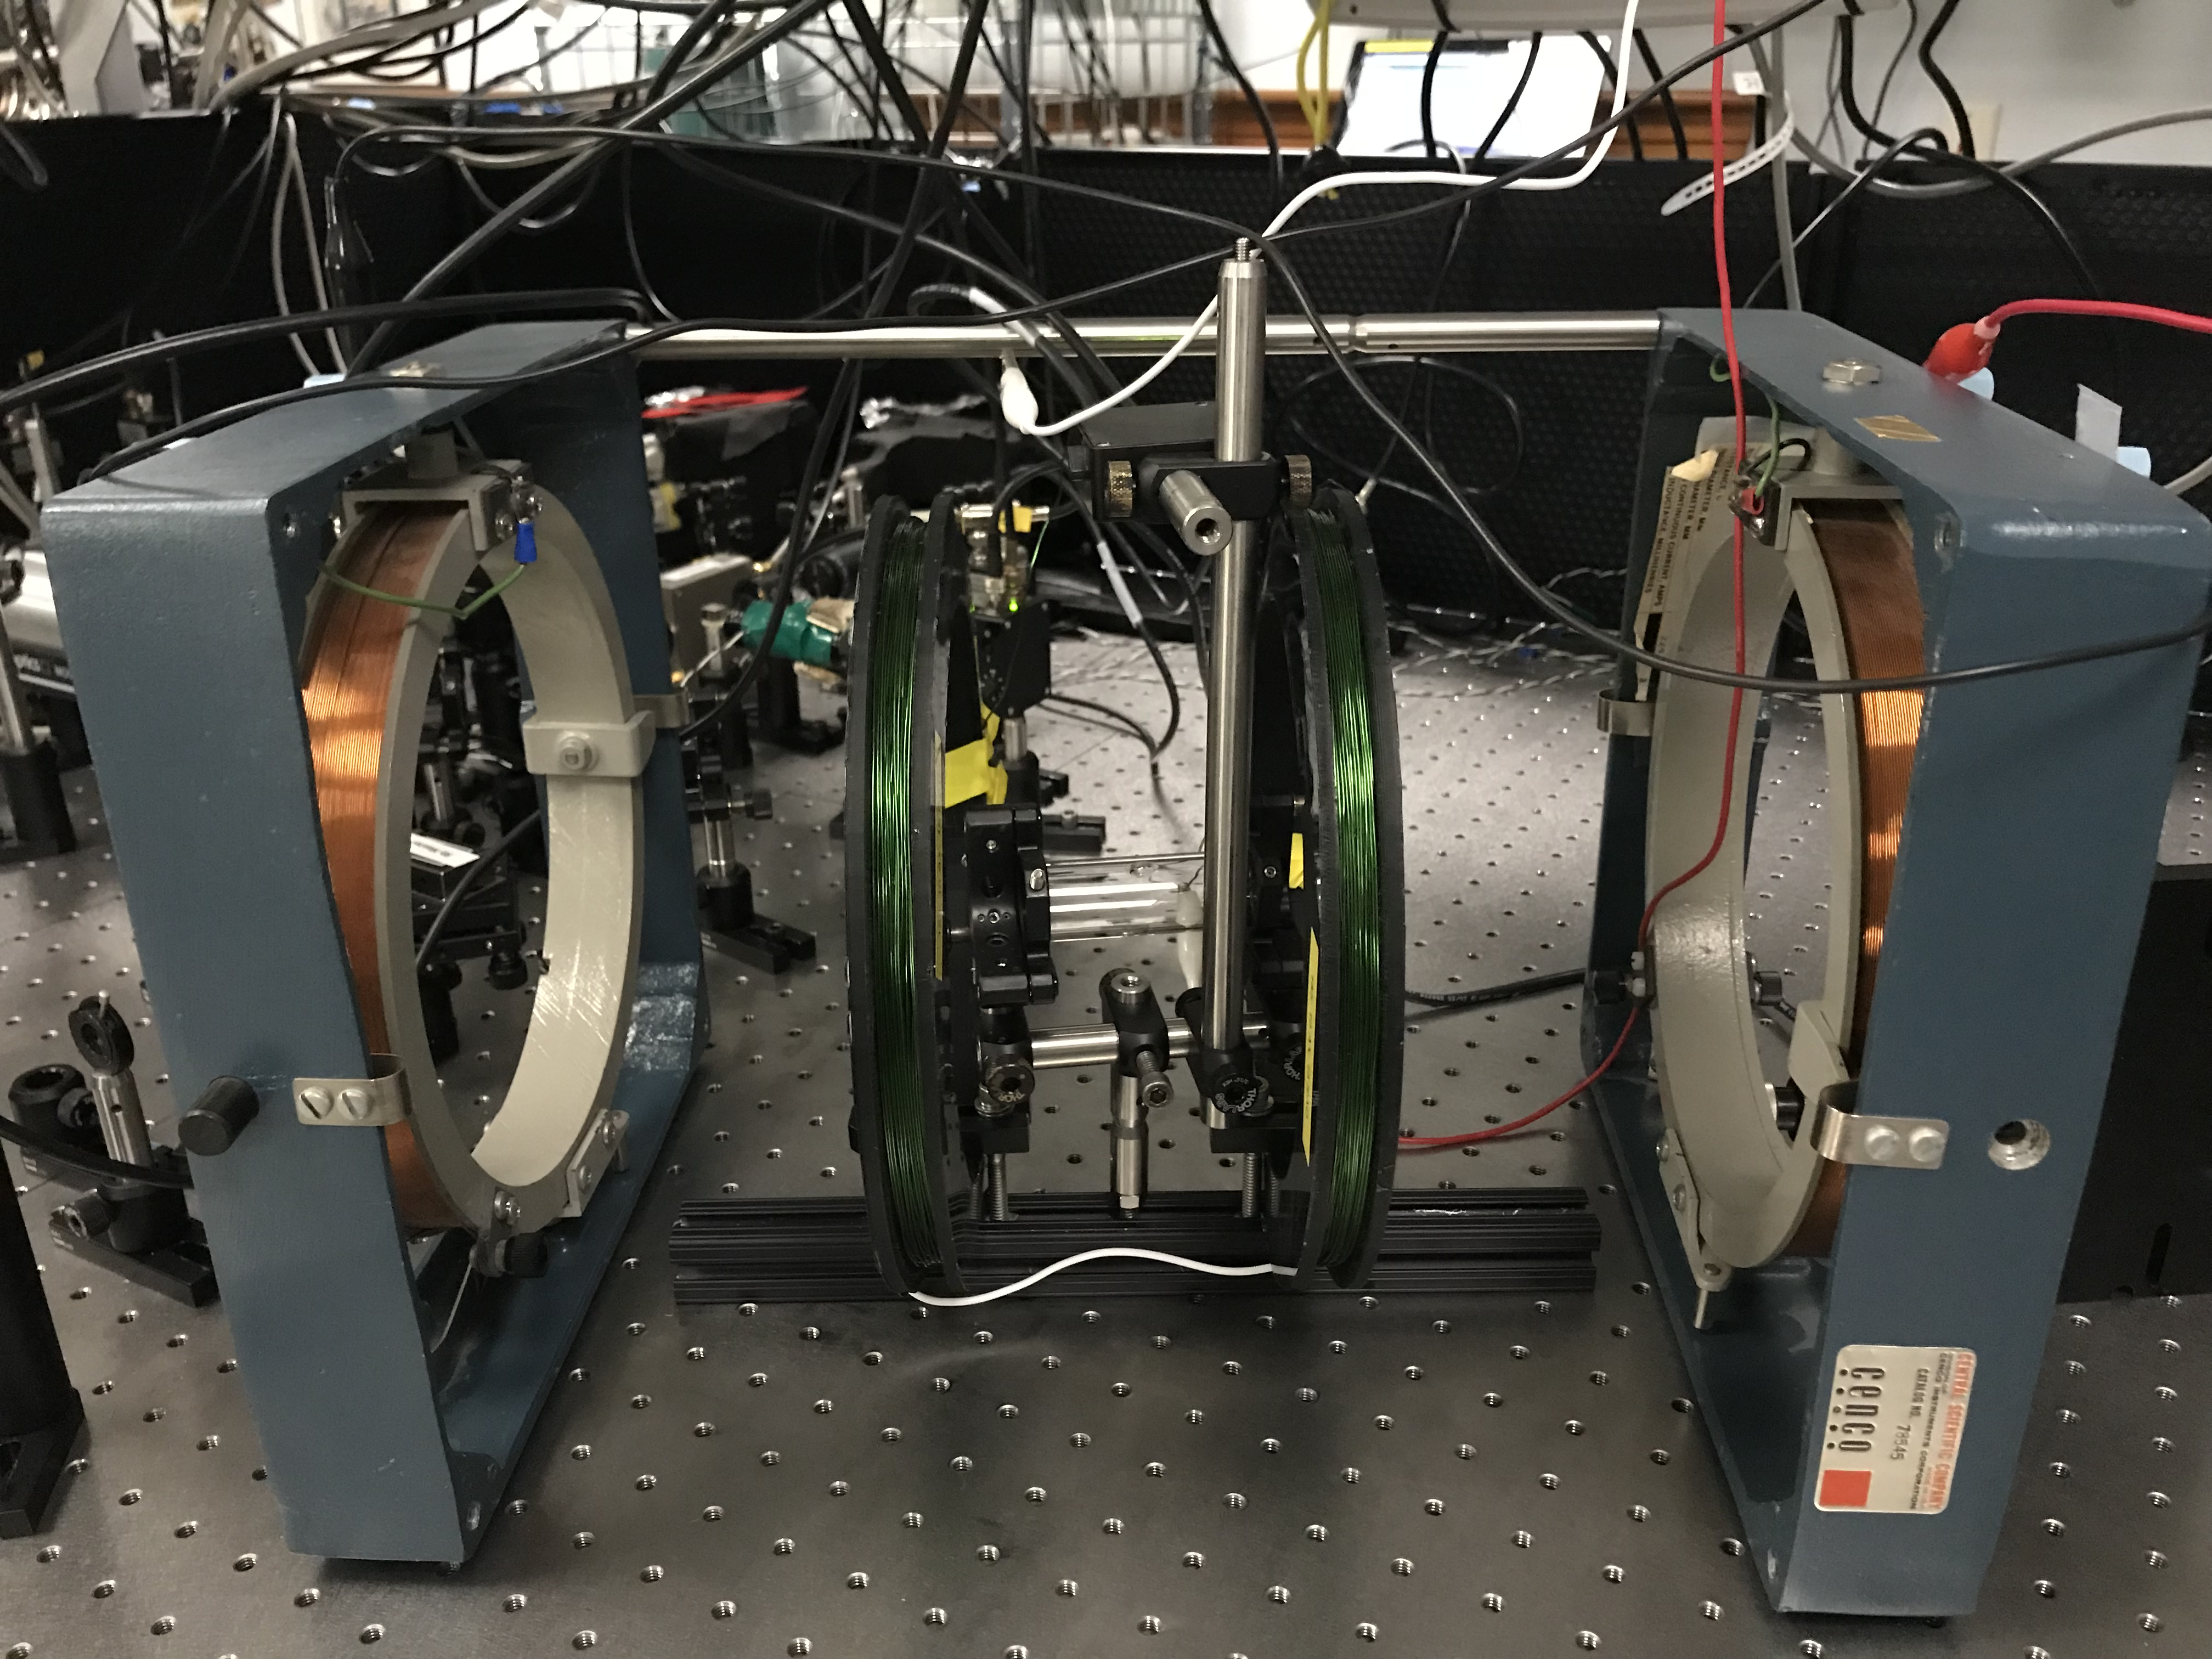
\includegraphics[width = .8\textwidth]{../Thesis/FullPaper/Images/actualcoils.png}
\end{frame}


%%%%%%%%%%%%%%%%%%%%%%%%%%%%%%%%%%%%%%%%%%%%%%%%%%
% FL versus Rep
%%%%%%%%%%%%%%%%%%%%%%%%%%%%%%%%%%%%%%%%%%%%%%%%%%

\begin{frame}{Fluorescence versus Repetition Rate of Laser}
	\centering
	\includegraphics[width = .9\textwidth]{../MRPData/MAR24/FLvrep.pdf}
\end{frame}

%%%%%%%%%%%%%%%%%%%%%%%%%%%%%%%%%%%%%%%%%%%%%%%%%%
% fl versus angle high
%%%%%%%%%%%%%%%%%%%%%%%%%%%%%%%%%%%%%%%%%%%%%%%%%%
\begin{frame}{Fluorescence versus Angle between Laser and Mag. Field}
	\framesubtitle{High Intensity}
	\centering
	\includegraphics[width = .85\textwidth]{../MRPData/MAR24/together.pdf}
\end{frame}

%%%%%%%%%%%%%%%%%%%%%%%%%%%%%%%%%%%%%%%%%%%%%%%%%%
% FL versus angle low
%%%%%%%%%%%%%%%%%%%%%%%%%%%%%%%%%%%%%%%%%%%%%%%%%%
\begin{frame}{Fluorescence versus Angle between Laser and Mag. Field}
	\framesubtitle{Low Intensity}
	\centering
	\includegraphics[width = .85\textwidth]{../MRPData/April16/together.pdf}
\end{frame}



%%%%%%%%%%%%%%%%%%%%%%%%%%%%%%%%%%%%%%%%%%%%%%%%%%
% Percent Changes in Fluorescence
%%%%%%%%%%%%%%%%%%%%%%%%%%%%%%%%%%%%%%%%%%%%%%%%%%
\begin{frame}{Percent Changes in Fluorescence}
\framesubtitle{}
\centering
\begin{minipage}{.49\textwidth}
\centering
	High Intensity
	\includegraphics[width=0.99\textwidth]{../MRPData/MAR24/togetherscaled.pdf}
\end{minipage}
\begin{minipage}{.49\textwidth}
\centering
	Low Intensity
	\includegraphics[width=0.99\textwidth]{../MRPData/April16/togetherscaled.pdf}
\end{minipage}
\end{frame}



%%%%%%%%%%%%%%%%%%%%%%%%%%%%%%%%%%%%%%%%%%%%%%%%%%
% Conclusion
%%%%%%%%%%%%%%%%%%%%%%%%%%%%%%%%%%%%%%%%%%%%%%%%%%
\begin{frame}
  \frametitle{Summary}
  \center
\begin{tikzpicture}[node distance = 1.75cm, auto]
    % Place nodes
    \node [block] (lgs) {Laser Guide Stars};
    \node [block, below of=op] (mrp) {Improving LGS with Magnetic Resonant Pulsing};
    \node [block, below of=mrp] (exp) {Our Experiment};
    % Draw edges
    %\path [line] (init) -- (identify);
	\draw[->, line width = 3pt] (lgs) -- (mrp);
	\draw[->, line width = 3pt] (mrp) -- (exp);
\end{tikzpicture}
\end{frame}



%%%%%%%%%%%%%%%%%%%%%%%%%%%%%%%%%%%%%%%%%%%%%%%%%%
% Question
%%%%%%%%%%%%%%%%%%%%%%%%%%%%%%%%%%%%%%%%%%%%%%%%%%
{\usebackgroundtemplate{\includegraphics[width=\paperwidth,height=\paperheight]{Images/ending_lgs.jpg}}
\begin{frame}
  \frametitle{Questions??}
  \vspace{6.5cm}
  \color{white}{\tiny ``Straight to the Milky Way's Heart,'' Scientific Computing, 2011}
\end{frame}}




%%%%%%%%%%%%%%%%%%%%%%%%%%%%%%%%%%%%%%%%%%%%%%%%%%
% Extras
%%%%%%%%%%%%%%%%%%%%%%%%%%%%%%%%%%%%%%%%%%%%%%%%%%
\begin{frame}{Extras}
  \framesubtitle{Subtitle}
		Slide Body
\end{frame}




%% Fourth Frame: Laser guide star: How to create a LGS
\begin{frame}
  \frametitle{Laser Guide Stars (LGS)}
  \framesubtitle{Sodium LGS}
  Sodium Laser Guide Star System
  \begin{itemize}
	\item Mesospheric sodium layer: 10 km thick and 90 km in altitude
	  \begin{itemize}
		\item Created by the ablation of meteors
	  \end{itemize}
  \end{itemize}
  \begin{minipage}{.45\textwidth}
  \begin{itemize}
	\item Wavelength $\lambda=$ 589.593 nm
	\item Intensity$^3$ $I \approx 10 Wm^{-2}$
	\item Circularly polarized light $\sigma ^+$
  \end{itemize}
\end{minipage}
\begin{minipage}{.35\textwidth}
  \begin{tikzpicture}
	\node at (0,0) {\includegraphics[width = 6cm, height = 3.5cm]{Images/sodium_emission.png}};
\end{tikzpicture}
\end{minipage}
	  %\bigskip
	 %\btVFill
	{\tiny $^3$Schock, M., et al. "Performance analysis of polychromatic laser guide stars used for wavefront tilt sensing." Monthly Notices of the Royal Astronomical Society 337.3 (2002)}
 
	  {\tiny Elvidge CD et al, ``Spectral identification of lighting type and character.`` Earth Observation Group}
\end{frame}



	%Sixth FRAME: DYE LASERS: SYSTEM OVERVIEW
\begin{frame}
  \frametitle{Our Experiment}
  \framesubtitle{Dye Lasers}
  \begin{itemize}
	\item Excellent tunability over close to one hundred nanometers
	\item Lasing medium: organic fluid dye solution 
	\item Pumping: Laser light excites dye solution
	\item Cavity: Two mirrors and a diffraction grating
	\item Diffraction grating allows wavelength to be selected
  \end{itemize}
  \begin{tikzpicture}
	\node at (0,0) {\includegraphics[width = 6cm, height = 3.5cm,center]{Images/dyelaser_hayley.png}};
	\node at (.8,1.5) [] {Dye Cell};
	%\draw [white, line width = 1.6pt] (0,1.3) rectangle (1.6, 1.8);
	\node at (2,-1.5) [green, line width = 1.6pt]  {Pump Beam};
	\node at (-2,1.5) [line width = 1.6pt]  {Grating};
\end{tikzpicture}
  \bigskip
  { \tiny``Construction of a Dye Laser for Use in Detecting Ultracold RbCa,'' Hayley Whitson, Willamette University, 2012`}

\end{frame}



%% Seventh Frame: Dye Lasers: Our dye laser
\begin{frame}
  \frametitle{Our Experiment}
  \framesubtitle{Our Dye Laser}
  \begin{itemize}
	\item Moya cavity creates lasing and minimizes spontaneous emission
	\item Two amplification cells intensify output beam
	\item Pump with kilohertz, picosecond pump beam
  \end{itemize}
  \begin{columns}
	\column{.5\textwidth}
\center	Dye laser schematic
	\begin{tikzpicture}
	  \node at (0,0) {\includegraphics[scale =.25,left]{Images/ND6K.png}};
	  \node at (0,0) [blue] {Cell};
	  \draw [blue,line width = 1.6pt] (.4,-.4) circle [radius = .3];
  \end{tikzpicture}
  \column{.5\textwidth}
  \center Moya cavity
  \begin{tikzpicture}
	\node at (0,0) {\includegraphics[height = 3cm, width = 4cm]{Images/moya_cavity.png}};
\end{tikzpicture}
  \end{columns}
 {\tiny `` ND6K User Manual,'' Contiuum Lasers, 1994}
\end{frame}



\begin{frame}
  \frametitle{Our Experiment}
  \framesubtitle{Absorption Measurements}
  \begin{itemize}
	\item Take absorption spectroscopy measurements
	  \begin{itemize}
		\item $\vec B$ along one direction
		\item Measure absorption as $\lambda$ changes
		\item Change direction of $\vec B$ and repeat
	  \end{itemize}
  \end{itemize}
  \begin{center}
		\begin{tikzpicture}
		  \node at (0,0) {\includegraphics[width = 8cm, height = 3cm]{Images/absorbtionspectroscopy2.png}};
		  \node at (-4.5,0) [rotate = 90] {\footnotesize Intensity};
		  \node at (0,-1.7) {\footnotesize Wavelength (nm)};
		  \onslide<2> {\draw [blue, line width = 1.6pt](.7,-1.3) rectangle (1.8,1.3);
		  \node at (1.8,1.9) [blue] {589.6 nm};}
	\end{tikzpicture}
  \end{center}
  {\tiny Michael Richmond, Rochester Institute of Technology, \textit{spiff.rit.edu/classes/phys440/lectures/curve}}
\end{frame}

\begin{frame}{Optical Pumping}
  \framesubtitle{}
  \centering
  \includegraphics[width=0.8\textwidth]{../Thesis/FullPaper/Images/tikz/opticalpumping.pdf}
\end{frame}





\end{document}

%% References
%% Background Image
%% Bishop, Brianna, ``Bringing New Life to Laser Guide Star,''Lawrence Livermore National Laboratory, June 2014

%% 4 LGS in sky
%%Gemini Observatory/AURA, gemini.edu, `` laser-Guide Star HD Videos and Images``


%% sodium emission graph
%% Elvidge CD et al, `` spectral identification of lighting type and character.``  Earth Observation Group

%% Dye laser: Hayley whitson
%% Whitson, Hayley, Senior Thesis, Willamette University, 2012

%% Moya Cavity 
%% Continuum ND6k Manual


%% Larmor precession
%% wikipedia larmor precession

%%Optical pumping
%% Spin polarization byoptical pumping, Colinear laser spectroscopy
